% This LaTeX was auto-generated from MATLAB code.
% To make changes, update the MATLAB code and export to LaTeX again.

\documentclass{article}

\usepackage[utf8]{inputenc}
\usepackage[T1]{fontenc}
\usepackage{lmodern}
\usepackage{graphicx}
\usepackage{color}
\usepackage{hyperref}
\usepackage{amsmath}
\usepackage{amsfonts}
\usepackage{epstopdf}
\usepackage[table]{xcolor}
\usepackage{matlab}
\usepackage[paperheight=795pt,paperwidth=614pt,top=72pt,bottom=72pt,right=72pt,left=72pt,heightrounded]{geometry}

\sloppy
\epstopdfsetup{outdir=./}
\graphicspath{ {./analysis_media/} }

\begin{document}

\matlabtitle{Analysis of Voltages}


\matlabheading{This program will perform statisticall analysis on a time series of voltages}

\begin{matlabcode}


v_measurements =  [21.2, 19.5, 20.1, 18.3, 17.7, 15.0, 21.9, 24.7, 23.1, 20.2, 16.3, 22.8, 18.4, 23.5, 21.1]
\end{matlabcode}
\begin{matlaboutput}
v_measurements = 1x15    
   21.2000   19.5000   20.1000   18.3000   17.7000   15.0000   21.9000   24.7000   23.1000   20.2000   16.3000   22.8000   18.4000   23.5000   21.1000

\end{matlaboutput}
\begin{matlabcode}

% (1) Minimum 
v_min = min(v_measurements)
\end{matlabcode}
\begin{matlaboutput}
v_min = 15
\end{matlaboutput}
\begin{matlabcode}
fprintf("Average Voltage: %.2f\n",v_avg)
\end{matlabcode}
\begin{matlaboutput}
Average Voltage: 20.25
\end{matlaboutput}
\begin{matlabcode}

% (2) Maximum
v_max = max(v_measurements)
\end{matlabcode}
\begin{matlaboutput}
v_max = 24.7000
\end{matlaboutput}
\begin{matlabcode}
fprintf("Max Voltage: %.2f\n",v_max)
\end{matlabcode}
\begin{matlaboutput}
Max Voltage: 24.70
\end{matlaboutput}
\begin{matlabcode}

% (3) Average
v_avg = mean(v_measurements)
\end{matlabcode}
\begin{matlaboutput}
v_avg = 20.2533
\end{matlaboutput}
\begin{matlabcode}
fprintf("Average Voltage: %.2f\n",v_avg)
\end{matlabcode}
\begin{matlaboutput}
Average Voltage: 20.25
\end{matlaboutput}
\begin{matlabcode}

% (4) Std. Deviation
v_std = std(v_measurements)
\end{matlabcode}
\begin{matlaboutput}
v_std = 2.7622
\end{matlaboutput}
\begin{matlabcode}
fprintf("Std. Deviation of Voltages: %.2f\n",v_std)
\end{matlabcode}
\begin{matlaboutput}
Std. Deviation of Voltages: 2.76
\end{matlaboutput}
\begin{matlabcode}

% (5) Median 
v_med = median(v_measurements)
\end{matlabcode}
\begin{matlaboutput}
v_med = 20.2000
\end{matlaboutput}
\begin{matlabcode}
fprintf("Median Voltage: %.2f\n",v_med)
\end{matlabcode}
\begin{matlaboutput}
Median Voltage: 20.20
\end{matlaboutput}
\begin{matlabcode}

% (6) Num. Values > Avg 
num_vals_greater_than_avg = sum(v_measurements>v_avg)
\end{matlabcode}
\begin{matlaboutput}
num_vals_greater_than_avg = 7
\end{matlaboutput}
\begin{matlabcode}
fprintf("Number of Voltage Values > %.2f: %.f\n",v_avg, num_vals_greater_than_avg)
\end{matlabcode}
\begin{matlaboutput}
Number of Voltage Values > 20.25: 7
\end{matlaboutput}
\begin{matlabcode}

% (7) Values > Avg 
v_greater_than_avg = v_measurements(v_measurements > v_avg)
\end{matlabcode}
\begin{matlaboutput}
v_greater_than_avg = 1x7    
   21.2000   21.9000   24.7000   23.1000   22.8000   23.5000   21.1000

\end{matlaboutput}
\begin{matlabcode}
fprintf("Voltage Greater than Average: %.2f\n", v_greater_than_avg)
\end{matlabcode}
\begin{matlaboutput}
Voltage Greater than Average: 21.20
Voltage Greater than Average: 21.90
Voltage Greater than Average: 24.70
Voltage Greater than Average: 23.10
Voltage Greater than Average: 22.80
Voltage Greater than Average: 23.50
Voltage Greater than Average: 21.10
\end{matlaboutput}
\begin{matlabcode}
% (8) Raw Plot 

plot(v_measurements)
title('Voltage Measurements')
xlabel('Sample #')
ylabel('Voltage')
\end{matlabcode}
\begin{center}
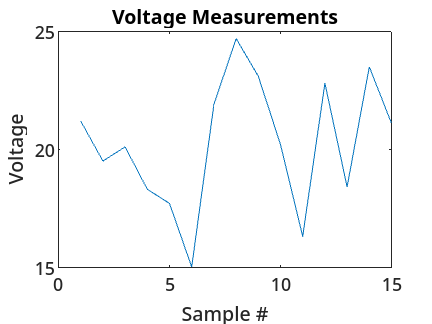
\includegraphics[width=\maxwidth{28.90115403913698em}]{figure_0.png}
\end{center}
\begin{matlabcode}

% (9) Histogram 
histogram(v_measurements)
title('Histogram of Voltages')
xlabel('Voltage')
ylabel('Occurances')
\end{matlabcode}
\begin{center}
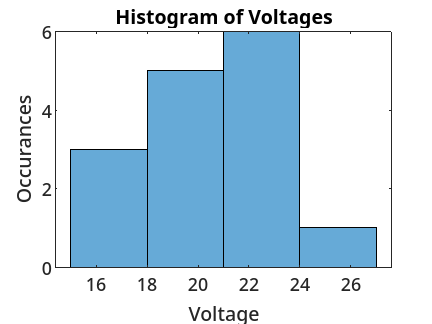
\includegraphics[width=\maxwidth{28.90115403913698em}]{figure_1.png}
\end{center}
\begin{matlabcode}

% (10) Sorted 
v_sorted = sort(v_measurements)
\end{matlabcode}
\begin{matlaboutput}
v_sorted = 1x15    
   15.0000   16.3000   17.7000   18.3000   18.4000   19.5000   20.1000   20.2000   21.1000   21.2000   21.9000   22.8000   23.1000   23.5000   24.7000

\end{matlaboutput}
\begin{matlabcode}

% printing sorted measurements in new lines 
disp("Voltages in sorted order: ")
\end{matlabcode}
\begin{matlaboutput}
Voltages in sorted order: 
\end{matlaboutput}
\begin{matlabcode}
for i = 1:length(v_sorted)
    fprintf("%.2f\n", v_sorted(i)); 
end
\end{matlabcode}
\begin{matlaboutput}
15.00
16.30
17.70
18.30
18.40
19.50
20.10
20.20
21.10
21.20
21.90
22.80
23.10
23.50
24.70
\end{matlaboutput}
\begin{matlabcode}

\end{matlabcode}

\end{document}
